\chapter{Tests}
\label{sec:test}
Folgendes Kapitel soll einen Überblick über die durchgeführten Tests geben und gegebenenfalls aufzählen welche Erkenntnisse aus diesen erlangt wurden.

\section{App}
\label{sec:appTest}

\subsection{Im Browser}

Beim Entwickeln der Oberfläche konnte die App im Browser getestet werden ohne diese dabei neu kompilieren zu müssen. Hier konnten zum Beispiel Tests für die verschiedenen Bildschirmgrößen durchgeführt werden.

\subsection{Als Windows App und im Android Emulator}

Für das Testen einiger Funktionen (z.B. Bluetooth) wird die Device-Umgebung benötigt. Hierfür wurde die Smartphone-App entweder als Windows App oder im Android Emulator getestet. So wurde zum Beispiel der Integrationstest zum Identity Server, bei dem spezielle Rechte für einen HTTP-Request benötigt werden, durchgeführt.

\subsection{Auf einem Endgerät}

Jedoch mussten viele Tests direkt auf dem Endgerät stattfinden. Die App kann dabei durch die im Chrome-Browser enthaltenen Debug-Features bestens, sogar über die IDE (z.B. VS-Code) \enquote{debugged} (siehe Abbildung \ref{fig:App_Debug_Device}) werden.

\begin{figure}[H]
	\begin{center}
		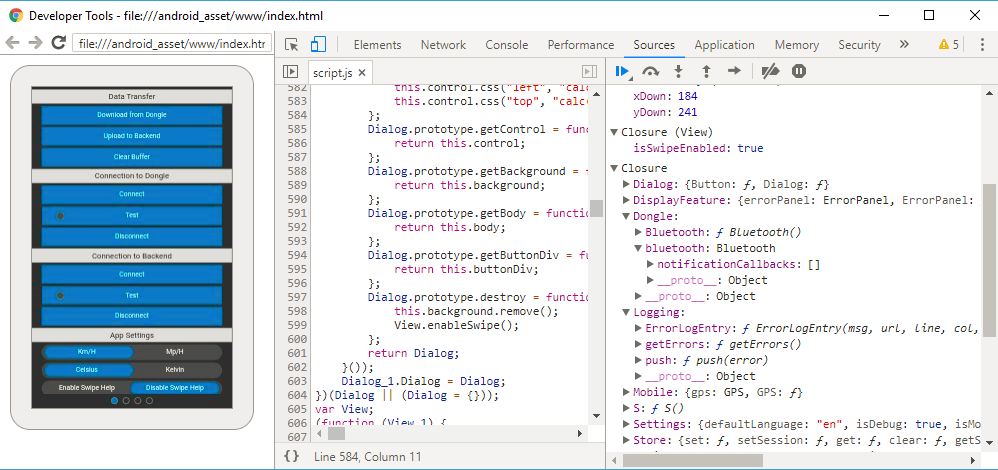
\includegraphics[height=7cm,keepaspectratio]{./img/App_Debug_Device}
		\caption{Debuggen der Smartphone-App auf Endgerät}
		\label{fig:App_Debug_Device}
	\end{center}
\end{figure}

\subsection{Während der Fahrt}

Da auch Fehler während der Fahrt auftreten können, hier jedoch nicht sofort auf diese eingegangen werden kann, werden diese mitprotokolliert und können nach der Fahrt ausgewertet und nachvollzogen werden. 



\section{Backend}
Nach dem Erreichen des geplanten Standes des Backends wurde dieses getestet. Hierfür wurden Trips unterschiedlicher Länge mehrfach in das Backend geladen. 

Bei diesen Tests wurde festgestellt, dass es eine schlechte Performance beim Interagieren mit den  Tracks gibt.
Beim Einlesen und erneuten Laden der Tracks, zum Beispiel für die Darstellung, wurde festgestellt, dass die benötigte Dauer fast unabhängig von der Größe des Tracks ist. Bei genauerer Recherche konnte festgestellt werden, dass die langen Zugriffszeiten durch den verwendeten Datenbankzugriff bedingt wurden. Dieser beruht auf \todo{@andi muss hier noch was ergänzen}%todo: sorry andi weis nicht genau was du damals gesagt hattest
Da es allerdings keine Alternative zu der verwendeten Technik gibt, konnte dieses Problem vorerst nicht gelöst werden.
	


\section{Dongle}
\label{sec:dongleTest}
Nach der erfolgreichen Integration der Dongle-Software erfolgte die Testphase, bei der der Dongle in iterativen Durchgängen an die OBD-Buchse verschiedener PKWs angeschlossen wurde. Hierbei wurden mehrere Fehlfunktionen entdeckt und behoben.
\paragraph{}
Es wurde zunächst deutlich, dass die Dauer der einzelnen Durchgänge der Haupt-Schleife weit über das erwartete Maß hinaus geht. Hierbei wurden die Zeitstempel zweier geloggter OBD-Werte mit der PID 0x0C verglichen. Dieser Wert ist der erste, der in jedem Durchgang erfasst wird. Folgende Werte zeigen beispielhaft die Dauern von Durchgänge bei denen alle Logging-Kategorien mindestens einmal erfasst wurden:
\begin{table}[htp!]
  \caption{Beispiel-Zeiten für einzelne Durchgänge der Haupt-Schleife}
  \label{tab:loopTimes}

  \begin{center}
    \begin{tabular}{|c|c|c|}
    \hline
      Durchgang & Dauer in Millisekunden & erfasste Logging-Kategorien\\ \hline
      0 & 488 & A\\ \hline
      1 & 708 & A + B\\ \hline
      2 & 960 & A + C\\ \hline
      3 & 608 & A + D\\ \hline
      4 & 656 & A + B\\ \hline
    \end{tabular}
  \end{center}
\end{table}
Eine Analyse zeigte auf, dass diese hohen Zeiten vor allem durch die Latenz bei der Abfrage der OBD-Daten vom Steuergerät zustande kommen. Dieses Verhalten kann nicht beeinflusst werden, stellt allerdings nur ein kleines Problem dar. Da zu jedem erfassten Wert auch ein Zeitstempel mit einer Genauigkeit von \textpm 8 Millisekunden gespeichert wird, ist die Einhaltung der angestrebten 500 Millisekunden für spätere Berechnungen nicht notwendig. Die Unterschiedliche Frequenz mit der die Logging-Klassen erfasst werden, welche mittels der Modulo-Operationen auf dem Loop-Counter erreicht wird, bleibt aufgrund der geringen Änderungsrate der Werte jedoch bestehen.
\paragraph{}
Darüber hinaus zeigten die Tests, dass die Verwendung des LowPowerModes des Coprozessors nicht den Erwartungen entsprach. Der STM32 konnte zwar in einen Schlafzustand versetzt werden, die Reaktivierung des selben konnte jedoch trotz intensiver Recherche im veröffentlichten Code und im offiziellen Freematics Forum nicht erreicht werden. Es zeigte sich allerdings, dass die verwendeten Funktionen aus den aktuelleren Versionen der offiziellen Softwarebibliotheken entfernt wurden \cite{freematicsRevFeb}. Da bereits ein Timeout bei der Abfrage von OBD-Werten dazu führt, dass die Dongle-Software ein Abstellen des Fahrzeuges vermutet, folgte daraus ein zufälliges Abbrechen der Aufzeichnung während einer laufenden Fahrt. Zur Beseitigung des Problems wurde auf die Verwendung des LowPowerModes verzichtet. Dieses Problem stellt im aktuellen Projektstand eine Verbesserungsmöglichkeit dar.
